\part{Model, View, Projection}
\frame{\partpage}

\begin{frame}{Model, View, Projection}
	\pause Drawing a 3D object on screen generally involves \textbf{three} transformations:
	\begin{itemize}
		\pause\item \textbf{Model}: translate, rotate and scale the object into its place in the scene
		\pause\item \textbf{View}: translate and rotate the scene to put the observer at the origin
		\pause\item \textbf{Projection}: convert points in 3D space to points on the 2D screen
	\end{itemize}
	\pause The \textbf{model-view-projection (MVP) matrix}:
		$$ M_{MVP} = M_{\text{projection}} \times M_{\text{view}} \times M_{\text{model}} $$
	(remember, multiplication goes in reverse order)
\end{frame}

\begin{frame}{The model matrix}
	\pause Exactly what we've been doing so far today...
\end{frame}

\begin{frame}[fragile]{The view matrix}
	\pause Need to translate and rotate the scene so that the ``camera'' is at $(0,0,0)$ and looking in the negative $z$ direction
	\pause\begin{lstlisting}
glm::mat4 view = glm::lookAt(
  glm::vec3(2, 0, 2),    // eye
  glm::vec3(0, 0, 0),    // centre
  glm::vec3 up(0, 1, 0)  // up
);
	\end{lstlisting}
	\begin{itemize}
		\pause\item \lstinline{eye} is the position of the camera
		\pause\item \lstinline{centre} is a point for the camera to look at
		\pause\item \lstinline{up} is which direction is ``up'' for the camera (usually the positive $y$-axis)
	\end{itemize}
\end{frame}

\begin{frame}{Types of projection}
	\pause\begin{center}
		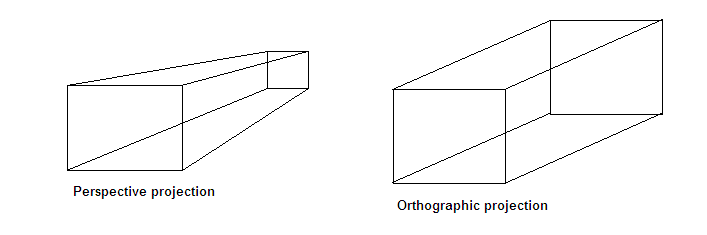
\includegraphics[width=\textwidth]{orthographic_perspective}
	\end{center}
	\begin{itemize}
		\pause\item Generally use \textbf{perspective} for 3D graphics
		\pause\item \textbf{Orthographic} is useful for 2D or pseudo-2D graphics (e.g.\ isometric perspective)
	\end{itemize}
\end{frame}

\begin{frame}[fragile]{The projection matrix}
	\pause\begin{lstlisting}
glm::mat4 projection = glm::perspective(
	glm::radians(45.0f), // field of view
	4.0f / 3.0f,         // aspect ratio
	0.1f,                // near clip plane
	100.0f               // far clip plane
);
	\end{lstlisting}
	\begin{itemize}
		\pause\item \textbf{Field of view (FOV)}: how ``wide'' or ``narrow'' the view is
		\pause\item \textbf{Aspect ratio}: should be \lstinline{screenWidth / screenHeight}
		\pause\item \textbf{Near and far clip planes}: fragments that fall outside this range of distances from the camera are not drawn
	\end{itemize}
	\pause Also available: \lstinline{glm::ortho} for orthographic projection
\end{frame}

\begin{frame}{The view frustum}
	\pause\begin{center}
		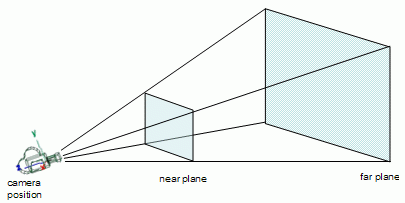
\includegraphics[width=0.8\textwidth]{frustum}
	\end{center}
	\begin{itemize}
		\pause\item Defined by the \textbf{near and far clipping planes} and the \textbf{edges of the screen}
		\pause\item \textbf{Nothing outside} the view frustum is visible
	\end{itemize}
\end{frame}

\begin{frame}[fragile]{Putting it together}
	\pause\begin{lstlisting}
glm::mat4 mvp = projection * view * modelTransform;
glUniformMatrix4fv(mvpLocation, 1, GL_FALSE, glm::value_ptr(mvp));
	\end{lstlisting}
	\pause And in the vertex shader, simply multiply the vertex position (in homogeneous coordinates) by the MVP matrix:
	\pause\begin{lstlisting}[language=GLSL]
uniform mat4 mvp;

void main()
{
  gl_Position = mvp * vec4(vertexPos, 1.0);
}
	\end{lstlisting}
\end{frame}
